Keywords: High performance computing, Energetic efficient systems, Power Modeling, Performance Modeling

\section{Description of the research project}

One of the main concerns regarding the construction and use of high-performance computing (HPC) systems is energy consumption. Currently, medium-size systems can consume hundreds of Kilowatts while high-end systems can reach dozens of Megawatts as we shown in figure \ref{fig:pw_consumption_a}. Maintain these systems are very expensive and depending on the energy resources they use it can also cause a huge Environmental impact. Also The next generation of HPC systems, the Exascale computing, capable of reaching a billion billion calculations per second, will be strongly constrained by their energy consumption as shown by the trend of the figure \ref{fig:pw_consumption_b}. Investigating new ways to reduce the energy consumption on HPC is crucial.

\begin{figure}[h]
    \centering
    \subfloat[Power consumption top 500 systems]{{
    \includegraphics[width=0.45\textwidth]{figures/power_rank.png} 
    \label{fig:pw_consumption_a}
    }}%
    \qquad
    \subfloat[Power by computational power]{{
    \includegraphics[width=0.45\textwidth]{figures/power_tflops.png}
    \label{fig:pw_consumption_b}
    }}%
    \caption{Power consumption}%
    \label{fig:pw_consumption}%
\end{figure}

Analyzing the contribution to the server power consumption we can see from the Google research \cite{Fan2007, Barroso2007} and also on my research at Federal University of Rio Grande do Norte on figure \ref{fig:cpu_util} that the processor is responsible for about 45\% of the total server power draw at peak usage being the main component responsible for the server power draw. Reducing the power consumption of the processor is very important in order to reduce the overall energy consumption.

\begin{figure}[h]
    \centering
    \subfloat[Power consumption top 500 systems]{{
    \includegraphics[width=0.45\textwidth]{figures/cpu_util.png}
    \label{fig:cpu_util_a}
    }}%
    \qquad
    \subfloat[Power by computational power]{{
    \includegraphics[width=0.45\textwidth]{figures/power_share.png}
    \label{fig:cpu_util_b}
    }}%
    \caption{Power draw on HPC}%
    \label{fig:cpu_util}%
\end{figure}

Modern processors incorporate several features for power management such as independent processing cores that can be enabled/disabled by the operating system \cite{Rotem2012}, clock gating techniques for reducing the dynamic power dissipation of synchronous circuits \cite{Srinivasan2015} and Dynamic Voltage and Frequency Scaling (DVFS) \cite{Mittal2014}. Besides that, there is also architectural approaches to reduce energy consumption including the use of simple but more power efficient processors, such as the ARM architecture used on smartphones, and also specialized architectures such as GPUs and FPGAs.


\subsection{Goals of the research}

The interest in developing this project is to make HPC increasingly viable, in addition to reducing maintenance costs and reducing the impact on the environment by saving energy.

Apart from this, our research also has international collaborations with other high-performance computing centers such as the Federal University of Rio Grande do Norte, where the project was started, and others which I had collaborated with projects related to energy saving in the University of Bristol, and possible future collaborations with University of Lausanne on Switzerland.

The main contribution of this thesis will be to produce better energy saving techniques for HPC based on dynamic models of applications’ performance, power/energy consumption analysis and extended DVFS techniques. As will be detailed in the next section, several objectives have been defined to address the multiple challenges of our proposal: consideration of the processor workload, instruction set and the input size of applications, more precise energy models based on additional execution parameters, alternative optimization strategies and automatization of the execution process.

First experiments developed showed that this methodology has a potential and can be improved to develop software as an end product that can be used by servers and clouds to save energy. This search can also be easily expanded to encompass mobile devices such as smartphones or microprocessed devices like raspberry-pi and beaglebone. Contributions in the areas of power consumption modeling and algorithms for frequency and voltage control off the processor are the product of this research.


\subsection{State of art}

DVFS has been demonstrated to be a very effective technique for reducing the power consumption of processors \cite{Hackenberg2015, Dzhagaryan2014, Hahnel2012, Basmadjian2012, Travers2015, Miyoshi2002, Anghel2011, Pietri2014}. The technique tries to optimize power consumption by adjusting the frequency according to the current load of the processor. Generally, the frequency scales with the intensity of the load and the voltage scales to the minimum value that enables the selected frequency. Among other aspects, DVFS helps reducing energy consumption because it allows memory-bounded programs to be executed more efficiently \cite{Spiga2006}. Nonetheless, aspects such as load variability may compromise the effectiveness of DVFS. Another important aspect that is typically not taken into account in DVFS is the number of processing cores to be used by a parallel program.

The DVFS technique has been extensively researched with the aim of providing strategies for selecting the optimal voltage and frequency for a specific application and architecture. In \cite{Anghel2011}, the authors used two algorithms for scaling the frequency of the processors: a human-immune system inspired algorithm to monitor the server's power and performance states, and fuzzy logic based algorithm for changing the server's performance state. \cite{Cochran2011} introduced a scaling method for determining the system's optimal operation points for the number of threads and DVFS settings. In \cite{DaCosta2015}, an approach that considers instantaneous system activity states was proposed. In this case, the memory and network activity were used to generate a DVFS management setting.

%In \cite{Georgiou:2017}, the authors used an energy model for a multi-threaded, multi-core embedded architecture and static resources analysis to statically evaluate the energy and timing savings of various DVFS configurations for the same program. Although, they were able to identify the most optimal configuration without the need of measuring time and energy of the program executed on each configuration alternative, this approach is quite limited, as static analysis does not scale to less time-predictable architectures and programs.

The use of energy measurements on the DVFS is stimulated by the large number of performance counters including on modern architectures providing a lot of debugging information on real-time including energy and power consumption information. These counters are accessed through the operating system via several interfaces.
Power models use to estimate power consumption of the CPU are based on the logic gates \cite{Du2017, Butzen2007}.  A logic gate consumes power mainly when it's changing state, and the frequency with which it changes state will probably be, on average, proportional to the clock frequency. In addition to leak current due to imperfection on the manufacture, basic models are generally:

\begin{equation}
    P_{cpu}=P_{dynamic}+P_{leak}+P_{static}
\end{equation}
and
\begin{equation}
    P_{dynamic} \quad \alpha \quad CV^2
\end{equation}

Where V is the voltage and f the operating frequency.

\subsection{Research project}

\subsubsection{Preliminary Work}

This proposal is based on my previous work on this topic as part of a master thesis where a develop a methodology to find optimal parameters for energy-frequency relations and the number of active cores needed to run single-node HPC applications using an application-agnostic power model of the architecture combined with an architecture-aware performance model of the application.

The power model used is based on CMOS (Complementary Metal-Oxide-Semiconductors) modeling, which are the intrinsic components of CPU chips. According to the operating frequency~\cite{Sarwar1997}, it models the dynamic, static and leakage power of the circuit. Besides operating frequency, the power model also parametrizes the number of active sockets and the number of active cores per-socket on a multi-core architecture:

\begin{equation}
    P(f,p,n)=(af^3+bf)p+cs+d
    \label{eq_power_final}
\end{equation}

Where $f$ is the frequency, $p$ is the number of active cores, $s$ the number of sockets on the system and $a$, $b$, $c$ and $d$ are constants.

% To fit the power-model equation, the CPU was stressed up to 100\% and power information was acquired on regular intervals. The coefficients of (\ref{eq_power_final}), $a$, $b$, $c$ and $d$, were found by performing multi-linear regression. The figure below shows the resulting fit for the system.

% \begin{figure}[H]
%     \centering
%     \includegraphics{image6.png}
%     \caption{Caption}
%     \label{fig:my_label}
% \end{figure}

The Performance is modeled by characterizing the application on the target architecture. The idea is to predict the performance of the application at any given configuration. The model takes as inputs the operating frequency, the number of active cores and the input size. The modeling is done using a supervised learning method for regression called Support Vector Regression (SVM)~\cite{Ventura2009, Smola2004} with data collected from multiple runs for different numbers of active cores, frequencies, and input sizes.

To find optimal-energy configurations, we can minimizes the product of outcomes of the power and performance models. Our approach was validated on four PARSEC applications~\cite{Bienia2008} and compared to the \emph{Ondemand} governor, which is the default DVFS scheme for the Linux operating system. The figure \ref{fig:previous_model} illustrates the entire process.

\begin{figure}[h]
    \centering
    \includegraphics[width=\columnwidth]{figures/old_model.png}
    \caption{Previous model}
    \label{fig:previous_model}
\end{figure}

% The figure below shows the energy equation for one specific input on one of the applications tested:
% \begin{figure}[H]
%     \centering
%     \includegraphics{image5.png}
%     \caption{Caption}
%     \label{fig:image5}
% \end{figure}

%This experiments was performed at High Performance Computing Center at the UFRN (NPAD/UFRN) using compute nodes that consists of two Intel Xeon E5-2698 v3 processors with sixteen cores each and two hardware threads for each core. The maximum non-turbo frequency is 2.2GHz, and the total physical memory of the node is 128GB (8$\times$16GB). The operating system used is Linux CentOS 6.5, kernel 4.16.9 Turbo frequency and hardware multi-threading were disabled during all experiments. 

%On the figure  \ref{fig:image5} we compare the proposed energy model with the real measured values.

% The steps need for this technique is:
% \begin{enumerate}
%     \item Run the power model fit once.
%     \item For each new application, run the performance model process.
%     \item Before the application start executing, use the power model and the performance model to compute the optimal energy configuration.
%     \item Set the frequency and disable cores according to the optimal values.
% \end{enumerate}

% All these steps can be performed without user intervention. The first step can be executed once the operating system is installed. The second step can be part of the installation process of the application, where the developer includes a configuration of how the application should be run and the operating system performs the process. The third and fourth are part of the operating system as a module. 

The use of an application-agnostic power modeling of the target architecture helps to make the technique portable to other applications. That is, to estimate the energy-optimal frequency and number of active cores for a new application, only a performance characterization is needed. In comparison with methods that only use information of processor workload, like the Linux default governor Ondemand, our technique has the disadvantage of including additional steps of performance characterizations. However, our results show that we are able to find configurations using about 14$\times$ less energy when compared to the worst case of the Ondemand governor. When compared to the best case of this DVFS scheme, i.e. when the user guesses the optimal number of cores to be used, the proposed approach was able to find configurations using up to 23\% less energy to run the target application. The overall average energy saving reached 6\% for the proposed approach when compared to the best case.

% \begin{figure}[H]
%     \centering
%     \includegraphics{image4.png}
%     \caption{Caption}
%     \label{fig:image4}
% \end{figure}

%The figure \ref{fig:image4} show the relative energy consumption for one application comparing to the Ondemand governor to multiples inputs. The application run on Ondemand with different number of cores.
The success obtained with this approach is probably due to the fact that the prior knowledge of the application's performance on the target architecture can expose sufficiently relevant information, such as parallel speedups, which are more difficult to guess with runtime techniques based on DVFS.


\subsubsection{Work continuation and motivation}

Although DVFS helps reduce system consumption, there are still cases where it is not effective or could be better. When there are abrupt variations in processor workload,  or when reducing frequency does not lead to less energy consumption, due to the program need to run for longer. This could be solved with prior knowledge of the application and power consumption of the system that we propose.

The currently proposed method still has some limitations: it optimizes the execution for only one application at a time, the execution frequency must be set at the beginning of the program execution, and the input used by the program must be known. In addition, the configuration mechanisms described in the previous section require a strategic integration with the operating system in order to be able to execute them automatically.

The input size can be estimated, allowing to consider alternative strategies when used as an optimization parameter. Combined with the previous model, that estimation will allow to split applications into execution stages and to apply the best optimization strategy at each stage. However, that estimation implies the identification of useful measurable parameters, such as CPU utilization, Cache Hit/Miss or memory utilization. 

There are still other alternatives to consider that deserve our attention. The previously proposed approach does not include frequency variations when running the application. Therefore, if the mathematical formulation can include this, it will be possible to find better results. Another parameter still not taken into account is that of the processor workload, which can bring a significant improvement to the power model. In addition to the inclusion of new parameters to the models, other models can still be proposed on mathematical formulation form or using, as in the case of SVR, learning methods. However, all this will require further analysis of the optimization alternatives that will appear in the benchmark tests as well as the study of the limits of each approach.

\subsection{Work plan}

Important points that will be addressed in this research:
\begin{enumerate}
    \item \textbf{Identify and analyzing important performance features for energy consumption}. Analyzing the application execution with multiple inputs on different configurations of active cores and frequencies, performance parameters and its relations can be chosen and associated to characterize the application. Since there is a large number of performance parameters, a study to select the principal components is necessary to reduce its complexity. 
    \item \textbf{Splitting the application into optimizable execution steps}. The goal is to split the application execution into several stages and minimize the energy on each stage, for that, the performance model is going to be completely remodeled. Creating a complete profile of the application, including performance parameters, frequency, and a number of active cores. With this, we can Cluster the applications identifying common frequency scaling stages to optimize. So when the application is running we can collect these performance features and find the closest cluster that will already have the optimized configuration.
    \item \textbf{Enhanced power models for HPC architectures: The power model is going to include additional parameters, such as the percentage of CPU utilization}. Further analysis of additional parameters, such as the influence of the instructions to be executed on the power consumed. Developing models that can reduce the overhead of training fitting and use fewer samples.
    \item \textbf{Enhanced DVFS models for HPC architectures: Including new architectures with distributed memory and heterogeneous systems}. Also studied the viability of using mathematical and artificial intelligence models, their advantages and their trade-offs to produce the final model. With these tools develops we can extend the current DVFS algorithms and produce a Smart DVFS module for HPC.
\end{enumerate}

The new workflow that we want to implement can be illustrated on the figures \ref{fig:new_model} and \ref{fig:heterogeneous_systems}.

\begin{figure}[h]
    \centering
    \includegraphics[width=\columnwidth]{figures/new_model.png}
    \caption{New model}
    \label{fig:new_model}
\end{figure}

\begin{figure}[h]
    \centering
    \includegraphics[width=\columnwidth]{figures/heterogeneous_systems.png}
    \caption{Heterogeneous systems}
    \label{fig:heterogeneous_systems}
\end{figure}

%\begin{figure}[h]
%    \centering
%    \includegraphics[width=\columnwidth]{figures/proposal.png}
%    \caption{Caption}
%    \label{fig:my_label}
%\end{figure}

% \newpage

% \section{Attachment}

% The figure below shows the resulting fit of the power model. To fit the power-model equation, the CPU was stressed up to 100\% and power information was acquired on regular intervals.

% \begin{figure}[H]
%     \centering
%     \includegraphics[width=10cm]{image6.png}
%     \caption{Power model fitting}
%     \label{fig:my_label}
% \end{figure}

% The energy model for one specific input for one of the applications tested is shown on the figure bellow
% \begin{figure}[H]
%     \centering
%     \includegraphics[width=10cm]{image5.png}
%     \caption{Energy model}
%     \label{fig:image5}
% \end{figure}

% The figure \ref{fig:image4} show the relative energy consumption for one application comparing to the Ondemand governor to multiples inputs. The application run on Ondemand with different number of cores.

% \begin{figure}[H]
%     \centering
%     \includegraphics{image4.png}
%     \caption{Comparison of the energy consumption of the proposed model to the Ondemand}
%     \label{fig:image4}
% \end{figure}


\section{Comments on changes made in the research project in case of resubmission(optional)}

Since the last submission, we have time to developed the first part of the project that was to collect performance counters a design a new application model that has a more precise definition of input size. The application architecture is shown on the figure \ref{fig:my_api}.

% \begin{figure}[h]
%     \centering
%     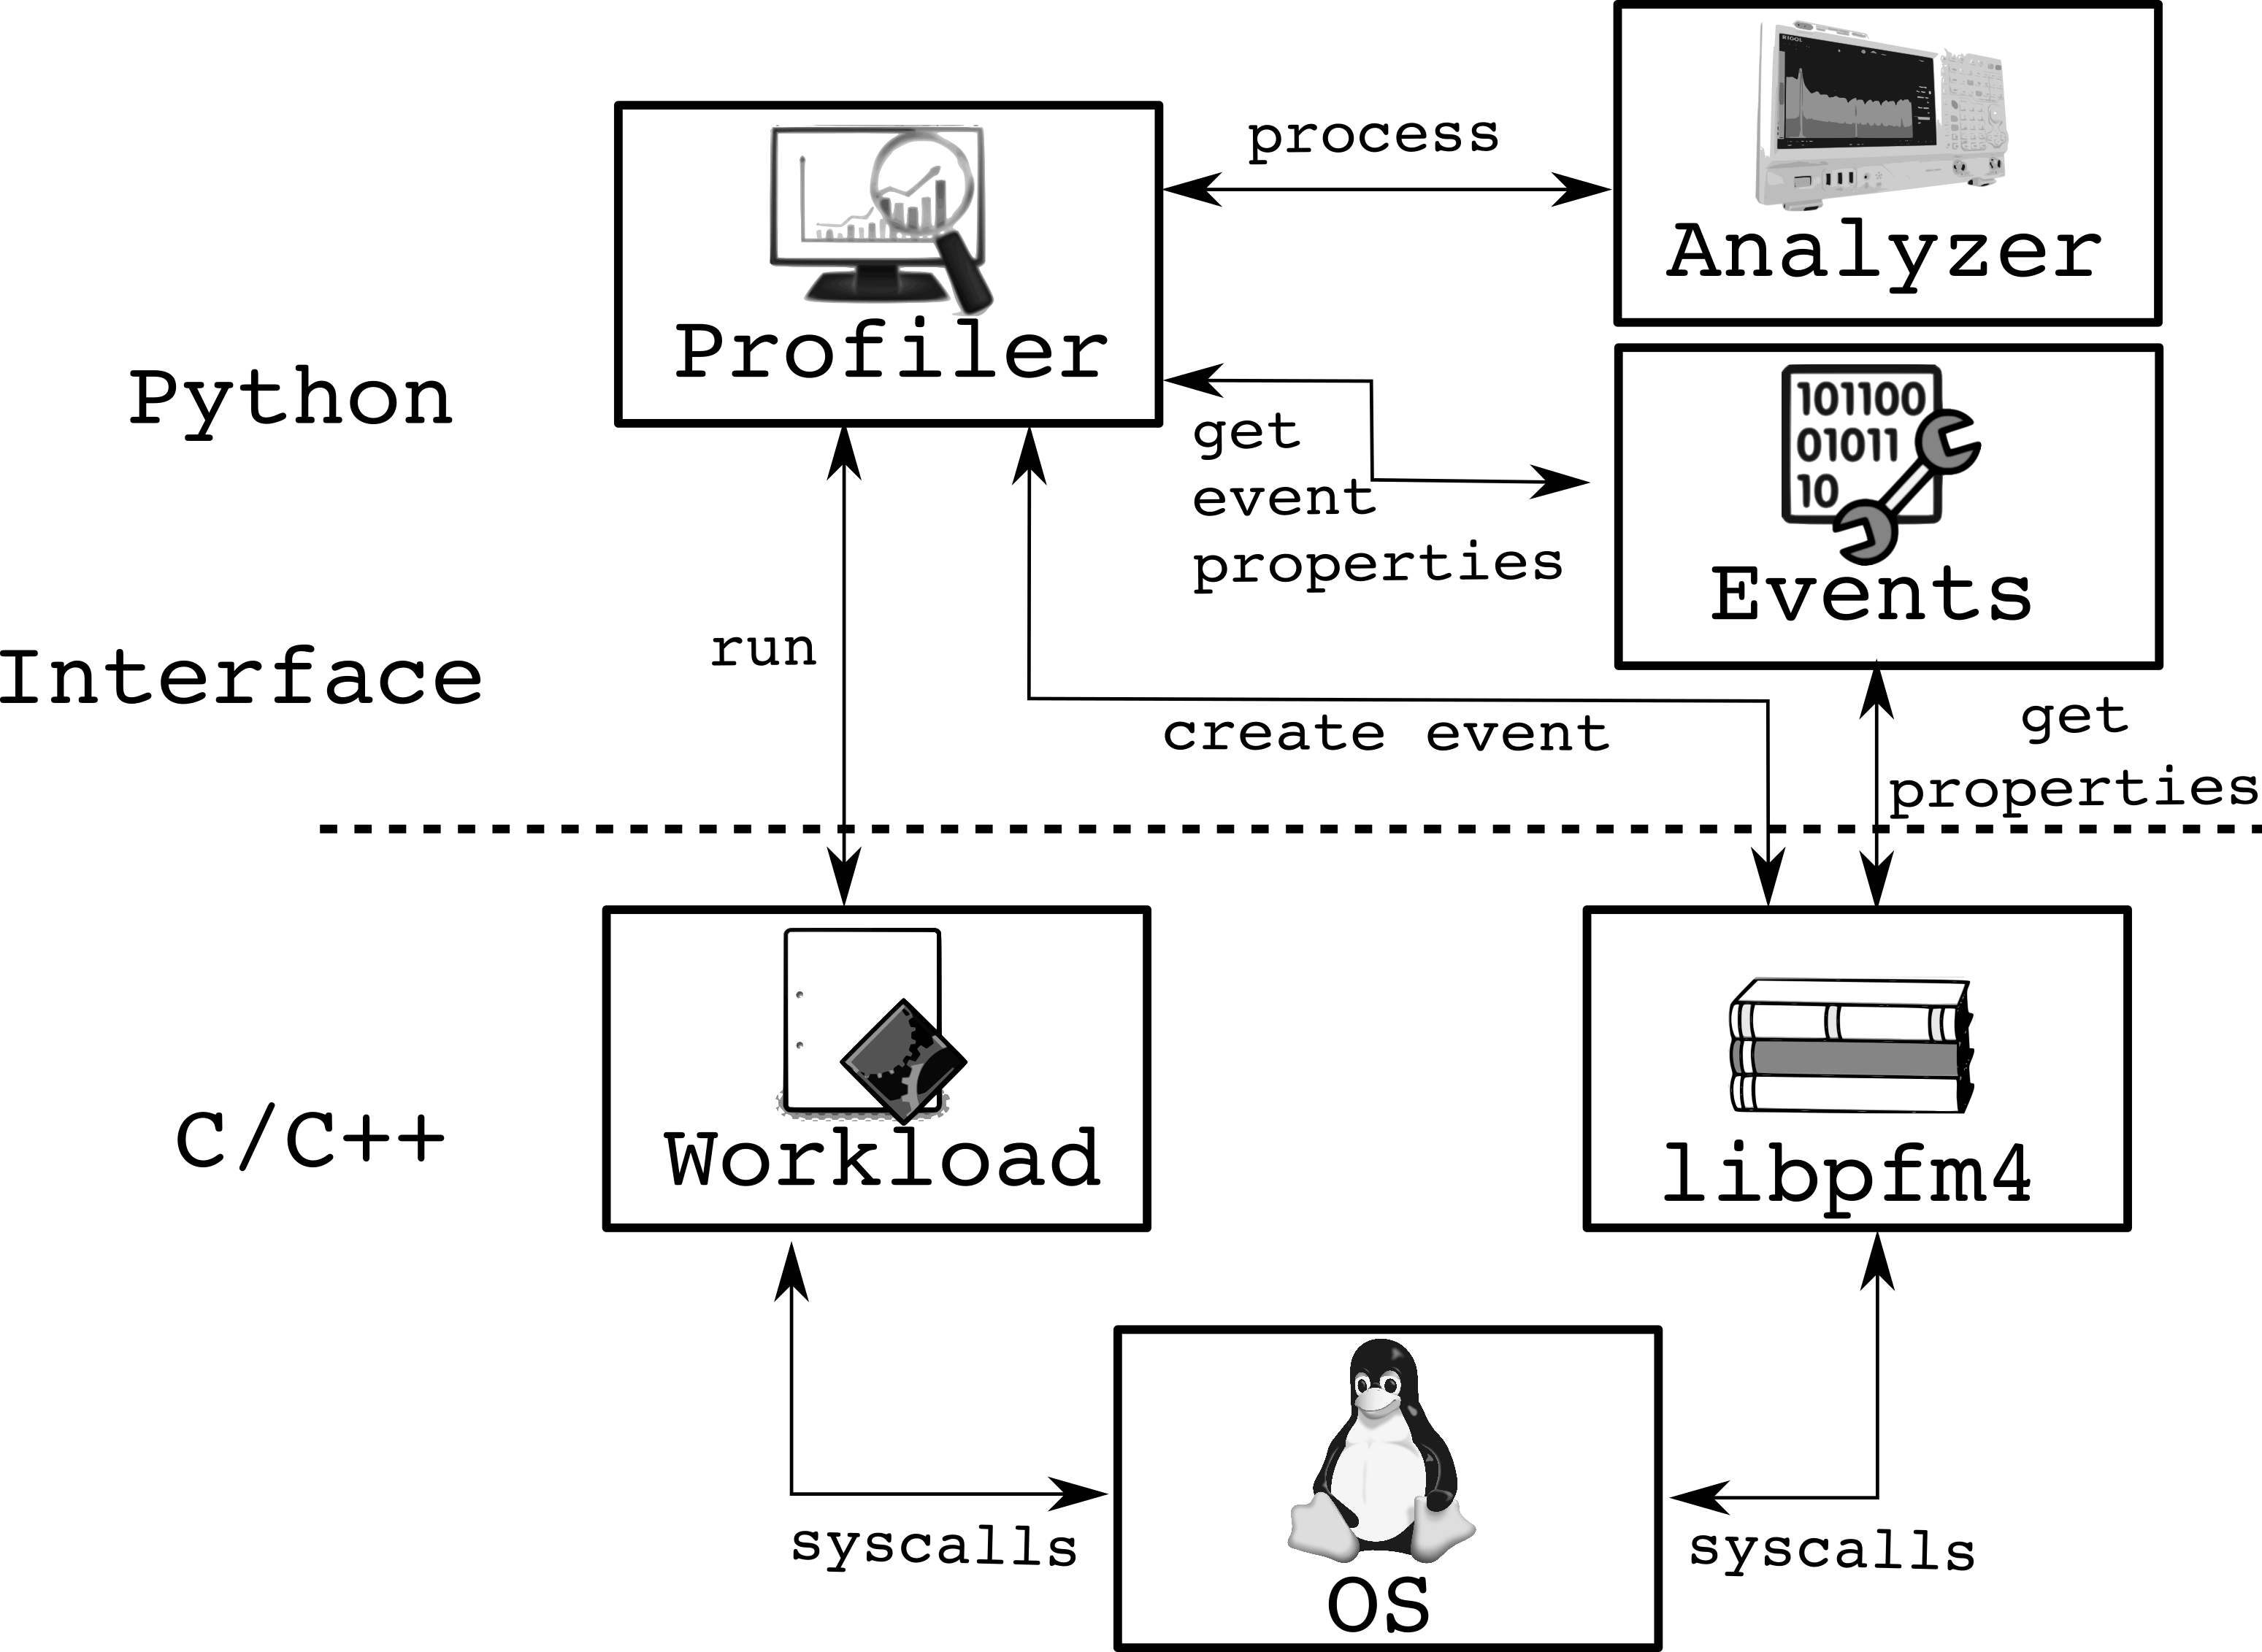
\includegraphics[height=7cm]{figures/architecture.png}
%     \caption{Tool developed to collect performance counters}
%     \label{fig:my_api}
% \end{figure}

\begin{figure}
    \subfloat[Architecture]{{
    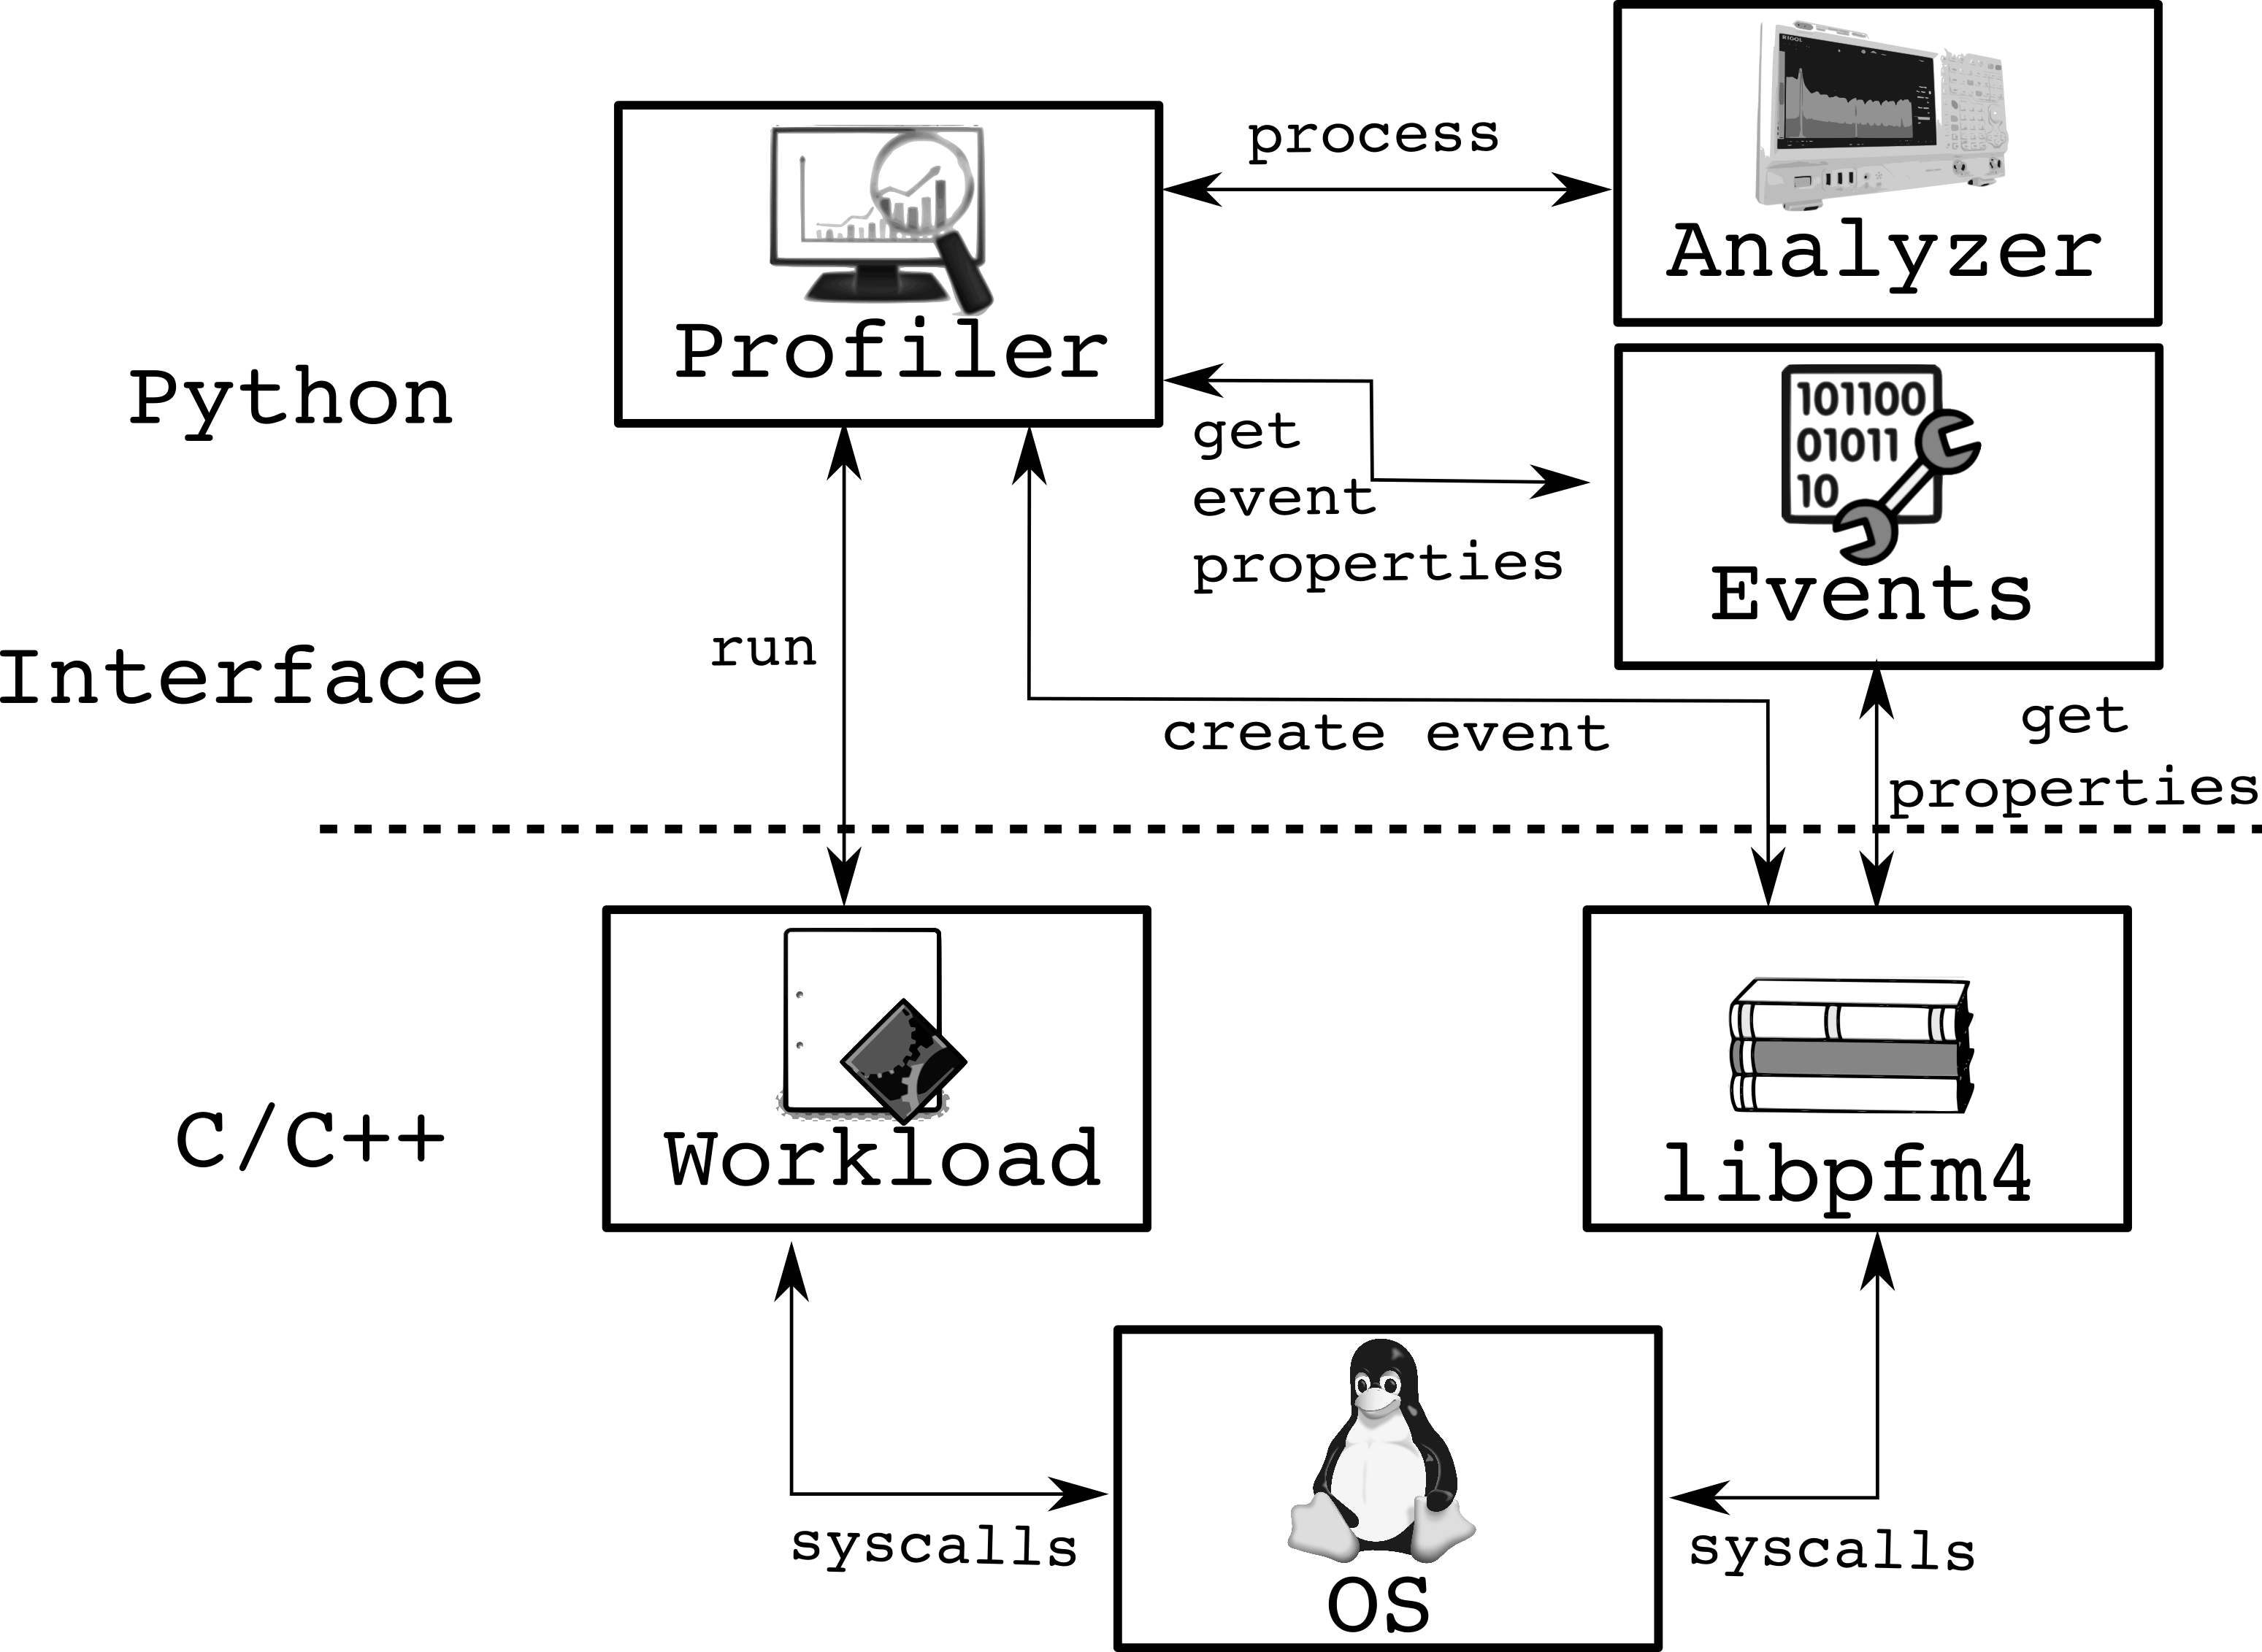
\includegraphics[width=0.45\textwidth]{figures/architecture.png}
    \label{fig:my_api}
    }}%
    \qquad
    \subfloat[Clusters]{{
    \includegraphics[width=0.45\textwidth]{figures/graph_input_size2.png}
    \label{fig:sping_force_is}
    }}%
    \caption{Tool to cluster applications}
\end{figure}

We develop a complete workflow to measure and prepossess the performance counters, the steps include running multiple times, remove outlines, interpolation, and filtering, we can see an example application on the figure \ref{fig:workflow}.

\begin{figure}[h]
    \centering
    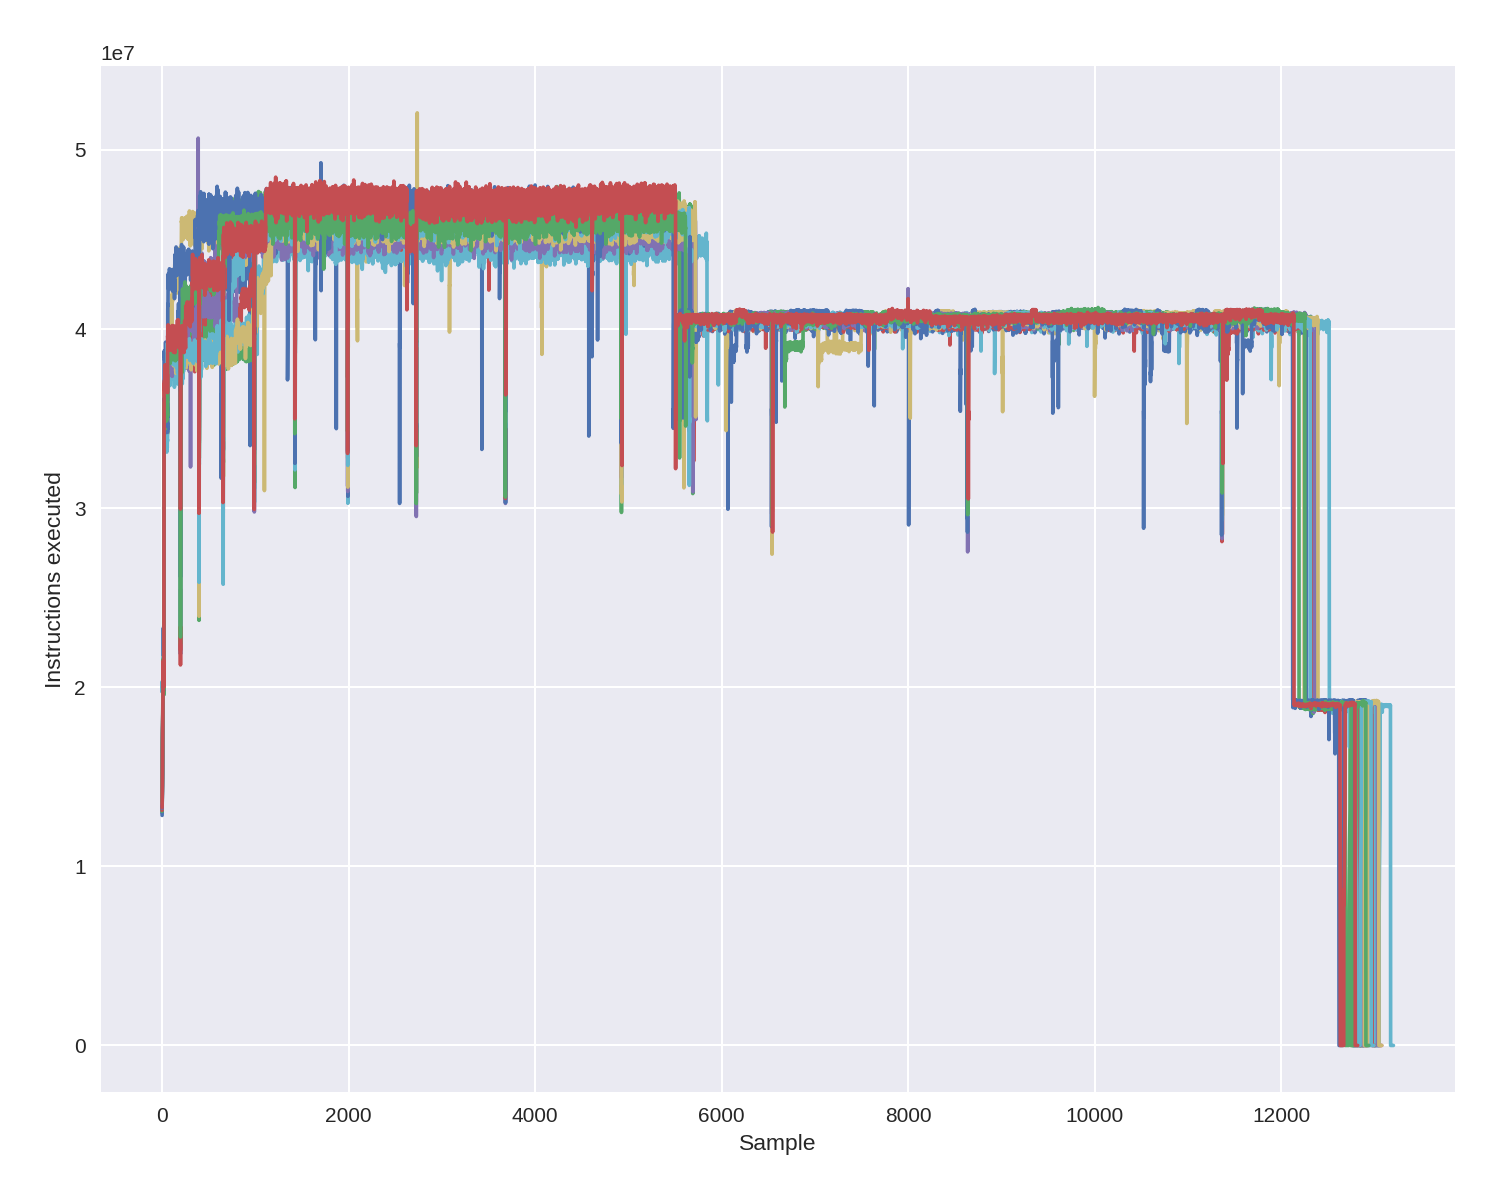
\includegraphics[width=\textwidth]{figures/workflow.png}
    \caption{Workflow}
    \label{fig:workflow}
\end{figure}

Finally we developed a new input size defined as:

\begin{equation}
I_{sz}=\frac{I_t}{I_m}*A
\end{equation}

Where $I_{t}$ is the total number of instructions, $I_m$ is the total number of memory instructions and A is the area of the original curve. This new input size can completely characterize the application execution and works as a fingerprint of the program so that we can proceed to the next step that is the clusterization.

On the figure, \ref{fig:sping_force_is} we display the clusters results that we obtain by comparing the input size curve of the PolyBench benchmark. An article describing the details of this first contribution was already submited to a conference and is waiting for approval.

\section{Activities report on the first year of doctorate}
ONLY for “1st grant - 2nd year” applicants

\section{Potential interdisciplinary approach of the research project (optional)}
This project involves Parallel and distributed computing, Operating system, Computer architecture, Programming, Mathematics, Physics, and Intelligent systems.

\section{Description of the work environment}
This research is developed in two HPC centers one at the host University, Faculte Polytechnique de Mons with a collaboration of the HPC center at Federal University of Rio Grande do Norte on Brazil (NPAD/UFRN). The environment is a supercomputer with multiple nodes, with 64 cores each, running a Linux system.

\section{Summary of the master’s thesis or equivalent}

This thesis proposes a methodology to minimize energy consumption in high-performance computing, finding the ideal frequency parameters and active cores in the processor. Based on a power modeling of the system, based on the power consumption of the CMOS circuit and an estimation of the execution time of the application using artificial intelligence, the energy equation is calculated as a function of frequency, number of cores and input of the application. With this equation, the configuration that minimizes the total power consumption is found. Tests were run on four applications and the results of this method showed that this approach achieved savings of up to 30\% when compared to the current energy-saving scheme on Linux.

\section{Additional comments (optional)}


\section{Ph.D. work calendar per month}

The above-mentioned objectives will be developed by following a structured work plan that will consist of the use of benchmarks, data collection and analysis, models proposal, experimental comparisons, and optimization steps. 

\begin{figure}[h]
    \centering
    \includegraphics[width=\columnwidth]{figures/workplan.jpg}
    \caption{Work plan}
    \label{fig:workplan}
\end{figure}
